\documentclass{Jurnal_kolo}
\usepackage[utf8]{inputenc}


%mengubah figure dan table menjadi bahasa Indonesia 
\usepackage[titles]{tocloft}
\renewcommand\cftfigpresnum{Gambar\  }
\renewcommand\cfttabpresnum{Tabel\   }


%Untuk Bold Face pada Keterangan Gambar
\usepackage[labelfont=bf]{caption}

%Untuk caption dan subcaption
\usepackage{caption}
\usepackage{subcaption}

\judul{KARAKTERISASI ASPEK AFEKTIF PERMUKAAN MENGGUNAKAN FITUR BERBASIS FOURIER TRANSFORM}
\penulis{Edi Setyawan Nugroho}
\afiliasi{Mohammad Faizun}
\prodi{Teknik Mesin}
\fakultas{Fakultas Teknologi Industri Universitas Islam Indonesia}
\alamat{Jl. Kaliurang Km. 14.5, Yogyakarta, Umbulmartani, Ngemplak, Kabupaten Sleman, Daerah Istimewa Yogyakara, 55584, Indonesia}
\email{16525070@students.uii.ac.id}
\emailaf{faizun@uii.ac.id}



\begin{document}
	\cetakheader
	\vspace{0.3 cm}
	\begin{abstract}
	\indent Penelitian ini dilakukan untuk  mengkarakterisasi aspek afektif pada sentuhan yang dihasilkan dari suatu permukaan material menggunakan fitur berbasis \emph{Fourier transform}. Di dalam penelitian ini terdapat tiga tahapan eksperimen. Eksperimen pertama adalah melakukan pengumpulan terminologi afeksi pada sentuhan dalam bahasa Indonesia. Hasil eksperimen menunjukkan bahwa terdapat dua jenis terminologi afeksi yaitu terkait dengan karakteristik fisik serta karakteristik emosi dari material tersebut. Pada eksperimen kedua adalah pemetaan afeksi sentuhan dari suatu permukaan pada bidang dua dimensi. Didapatkan hasil yang menunjukkan bahwa dimensi afeksi dingin-hangat dan keras-lembut tidak terlalu sesuai untuk diproyeksikan pada bidang dua dimensi. Diduga bahwa kedua dimensi afeksi ini akan optimal apabila diproyeksikan pada bidang tiga dimensi. Eksperimen ketiga adalah pembuatan model \emph{machine learning} untuk mengetahui hubungan afeksi dengan fitur berbasis \emph{Fourier transform}. Performa model diukur menggunakan nilai akurasi dan kurva ROC. Hasil pengujian performa dengan nilai akurasi menunjukkan bahwa model lemah dalam melakukan klasifikasi permukaan pada dimensi afeksi keras-lembut (59.09 \%) dan dingin-hangat (68.18\%). Sedangkan model memiliki performa paling baik dalam melakukan klasifikasi dimensi afeksi nyaman-sakit dengan akurasi 93.18 \%.\\
	\noindent
	\textbf{Kata kunci :} \emph{Machine Learning}, \emph{Multidimensional Scaling}, \emph{Fourier transform}, Afeksi, \emph{Affective Engineering}.
	\end{abstract}

\setlength{\columnsep}{1cm}
\begin{multicols}{2}
	\section{Pendahuluan}
	Dewasa ini banyak produsen dari suatu produk yang mulai menjadikan hal-hal non-teknis seperti estetika, afeksi dan kenyamanan sebagai salah satu pertimbangan utama dari produk yang mereka buat. Hal ini dikarenakan pihak produsen sendiri ingin membuat suatu produk yang dapat menimbulkan ikatan emosional dengan penggunannya \cite{Bahn2009}\cite{Khalid2006}. Salah satu aspek agar ikatan emosional antara produk dengan pengguna adalah dengan sentuhan.\\
	\indent Tekstur dari suatu permukaan produk mempunyai peran yang penting dalam terciptanya kesan emosional dari suatu produk melalui sentuhan. Ini dikarenakan tekstur merupakan suatu fitur penting yang digunakan manusia untuk memperoleh informasi melalui sentuhan. Dunia industri saat ini berusaha untuk membuat produk mereka memiliki tekstur yang dapat menimbulkan kesan emosional pada pengguna seperti yang mereka inginkan. \\
	\indent Saat ini perancangan dan riset dari tekstur permukaan yang dapat menimbulkan kesan emosional tertentu pada manusia menggunakan metode \emph{trial and error}. Hal ini tentunya sangat merugikan produsen mengingat memakan banyak waktu dan biaya. Ini memicu banyak penelitian terkait pendekatan saintifik untuk menentukan tekstur suatu permukaan yang dapat menimbulkan kesan emosional tertentu pada manusia. Salah satu alternatif yang ditawarkan oleh penulis adalah dengan mengidentifikasi karakteristik aspek afektif dari permukaan menggunakan fitur berbasis \emph{Fourier transform}. 
	\section{Metodologi}
	
	\begin{figure}[H]
		\centering
		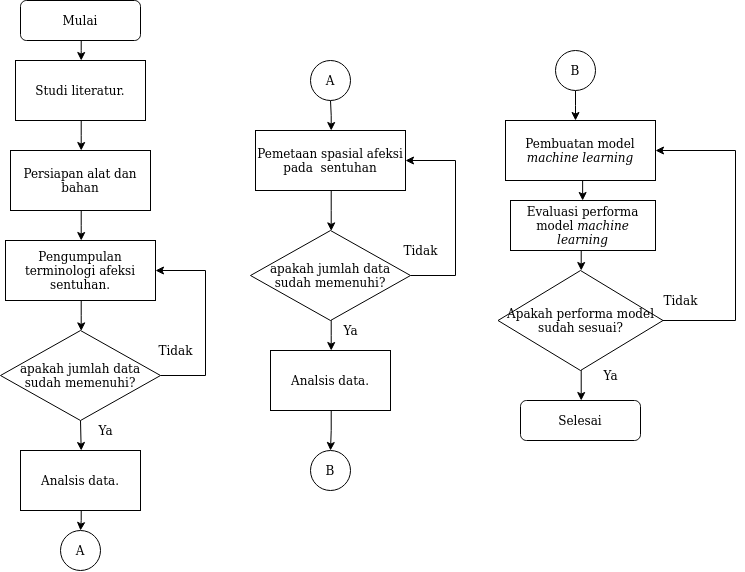
\includegraphics[scale=0.3]{gambar/alurjurnal}
		\caption{Alur penelitian.}
		\label{alur}
	\end{figure} 
	
	\subsection{Pengumpulan Terminologi Afeksi}
	\subsubsection{Subjek}
	\indent Subjek eksperimen ini terdiri atas 24 (13 perempuan dan 11 laki-laki) warga negara Indonesia dengan rentang umur 20 sampai dengan 25 tahun. Semua subjek bersifat naif. Naif yang dimaksud adalah semua subjek belum pernah mengetahui atau berpartisipasi pada eksperimen serupa sebelumnya.\\
	\subsubsection{Sampel}
	\indent Pada eksperimen ini digunakan sampel berupa beberapa jenis material untuk disentuh oleh subjek. Digunakan sampel berupa kulit sintetis, kain bludru, kertas amplas 80 dan kertas amplas 150. Bagian belakang dari kulit sintetis dan kain bludru juga digunakan karena memiliki tekstur yang cukup unik.   
	\subsubsection{Prosedur}
	\indent Terdapat beberapa langkah utama dalam pelaksanaan eksperimen ini. Langkah pertama sosialisasi mengenai protokol percobaan dan penandatangan \emph{concern form} oleh subjek penelitian. Hal ini dilakukan untuk menginformasikan kepada subjek mengenai eksperimen yang dilakukan dan hal-hal yang harus dilakukan oleh subjek. Selanjutnya adalah subjek diminta untuk menyentuh spesimen uji yang sebelumnya telah disiapkan menggunakan jari manis tangan dominan. Pada tahap ini dikondisikan supaya subjek tidak melakukan kontak visual dengan spesimen uji ketika menyentuhnya menggunakan kotak penutup. Setelah menyentuh spesimen uji, subjek diminta untuk melaporkan kesan apa saja yang dirasakan. Langkah ini diulangi sampai dengan semua spesimen uji dapat disentuh oleh subjek. Urutan pemberian spesimen uji diacak dan dibuat sehingga setiap subjek merasakan spesimen uji dengan urutan yang berbeda.
	
	\subsection{Pemetaan Spasial Afeksi Pada Sentuhan}
	\subsubsection{Subjek}
	\indent Subjek eksperimen ini terdiri atas 20 (10 perempuan dan 10 laki-laki) warga negara Indonesia dengan rentang umur 20 sampai dengan 25 tahun. Semua subjek bersifat naif. Naif yang dimaksud adalah semua subjek belum pernah mengetahui atau berpartisipasi pada eksperimen serupa sebelumnya.
	
	\subsubsection{Sampel}
	\indent Pada eksperimen pemetaan spasial afeksi pada sentuhan ini digunakan 11 jenis material yang berbeda. Material tersebut diantaranya adalah Kayu, Kain Goni, Kertas Amplas 150, bludru, \emph{Wax Paper}, Nilon, kulit sintetis, \emph{Cellulose Sponge}, Plastik, Karet Penghapus dan \emph{Polyfoam}.
	
	\subsubsection{Prosedur}
	\indent Prosedur kerja dari eksperimen terdiri atas beberapa langkah utama. Langkah pertama pembacaan protokol percobaan dan penandatangan \emph{concern form} yang merupakan bukti persetujuan bahwa subjek bersedia mengikuti seluruh protokol percobaan yang ada. Selanjutnya subjek diminta untuk menyentuh spesimen uji yang telah disiapkan menggunakan jari manis tangan dominan. Ketika menyentuh spesimen uji subjek dikondisikan untuk tidak dapat melakukan kontak visual dengan spesimen uji. Setelah menyentuh spesimen uji subjek diminta untuk menentukan skala yang menunjukkan tingkat dari afeksi yang dirasakan. Langkah ini diulangi sampai dengan semua spesimen uji dapat disentuh oleh subjek. Urutan pemberian spesimen uji diacak dan dibuat sehingga setiap subjek merasakan spesimen uji dengan urutan yang berbeda.
	
	\subsection{Pembuatan Model \emph{Machine Learning} Karakteristik Afeksi}
	\subsubsection{Subjek}
	\indent Subjek eksperimen ini terdiri atas 5 laki-laki warga negara Indonesia dengan rentang umur 20 sampai dengan 25 tahun. Semua subjek bersifat naif. Naif yang dimaksud adalah semua subjek belum pernah mengetahui atau berpartisipasi pada eksperimen serupa sebelumnya.
	
	\subsubsection{Sampel}
	\indent Pada pembuatan model \emph{machine learning} karakteristik afeksi digunakan dua jenis material sebagai sampel. Material tersebut adalah kain \emph{suede} dan bulu sintetis. Kedua sampel digunakan untuk melakukan survey kepada subjek dalam upaya untuk melakukan validasi dari model yang dibuat.
	
	\subsubsection{Prosedur}
	\indent Pada eksperimen ini digunakan data hasil survey yang sebelumnya telah dilakukan. Total terdapat 220 data berhasil dikumpulkan dari 20 subjek yang menyentuh 11 spesimen uji. Data tersebut akan digunakan sebagai data target. Sedangkan data berupa fitur \emph{Fourier transform} hasil ekstraksi dari citra digital permukaan material akan digunakan sebagai data prediktor. Proses ekstraksi fitur dilakukan menggunakan program yang ditulis menggunakan bahasa dan \emph{library} Python. Fitur berbasis \emph{Fourier transform} yang digunakan adalah sebanyak 109 buah fitur. Kedua data tersebut dibagi menjadi dua dengan proporsi data latih 80\% dan data uji 20\% dari total data yang ada.\\	
	\indent Data yang diperoleh dari hasil survey digunakan sebagai target atau output dari model. Data tersebut masih berbentuk skala 1 sampai dengan 5 yang merepresentasikan tingkat afeksi yang muncul. Untuk membuat data target, data yang sebelumnya masih dalam bentuk skala dengan rentang 1 sampai dengan 5 diubah menjadi 1 dan 0. Dimana 0 merepresentasikan nilai batas yang telah ditentukan sampai dengan nilai 1 sedangkan nilai 1 pada data target merepresentasikan nilai batas yang ditentukan sampai dengan nilai 5 pada data hasil percobaan sebelumnya. Nilai skala yang dijadikan nilai batas oleh peneliti adalah 3. Sehingga nilai lebih kecil dari 3 akan diubah menjadi 0 sedangkan untuk nilai lebih dari 3 diubah menjadi 1 secara otomatis oleh fungsi \emph{Binarization} pada \emph{library}  scikit learn.\\
	\indent Untuk data prediktor juga dilakukan beberapa praproses sebelum digunakan sebagai data latih dan data uji. Pertama, data prediktor dilakukan proses standarisasi. Ini dikarenakan fitur berbasis \emph{Fourier transform} memiliki skala dan satuan yang berbeda. Setelah itu data fitur hasil normalisasi dilakukan proses pemilihan fitur. Proses ini dilakukan dengan tujuan untuk mengeliminasi fitur yang saling linear. Ini dikarenakan fitur yang saling linear dikhawatirkan dapat menganggu performa dari model.\\
	\indent Data hasil pra proses dibagi menjadi data latih dan data uji. Untuk proporsi data latih adalah 80\% dari total data dan data uji adalah 20\%. Data latih digunakan untuk melatih model \emph{machine learning}. Model \emph{machine learning} yang dipilih adalah \emph{Multi-Output Logistic Linear Regression}. Alasan pemilihan model ini adalah kesesuaian dengan kasus yang dihadapi yaitu melakukan klasifikasi dan prediksi secara bersamaan.\\
	\indent Model lalu akan dilakukan validasi dengan survey menggunakan spesimen uji yang telah disiapkan sebelumnya. Spesimen uji validasi diekstraksi fitur berbasis \emph{Fourier transform} lalu dimasukkan kedalam model untuk diprediksi afeksi yang dapat muncul dari kedua spesimen tersebut. Hasil prediksi menggunakan hasil survey.
	
	
	\section{Hasil}
	\subsection{Pengumpulan Terminologi Afeksi}
	\indent Pada eksperimen ini ditemukan adanya 19 terminologi terkait dengan afeksi pada sentuhan. Dikarekankan beberapa terminologi yang muncul frekuensinya sangat rendah maka dilakukan seleksi pada terminologi yang muncul. Berikut adalah hasil berupa terminologi yang berhasil diseleksi.
	
	\begin{table}[H]
		\centering
		\caption{\label{tab-termi}Daftar terminologi afeksi.}
		\begin{tabular}{|c|c|c|}
			\hline
			No. & Terminologi & Frekuensi Kemunculan\\
			\hline
			1 & Halus & 47\\
			\hline
			2 & Kasar & 49\\
			\hline
			3 & Nyaman & 15\\
			\hline
			4 & Enak & 13\\
			\hline
			5 & Lembut & 25\\
			\hline
			6 & Hangat & 5\\
			\hline
			7 & Kesat & 22 \\
			\hline
			8 & Licin & 20\\
			\hline
			9 & Bertekstur & 31\\
			\hline
			10 & Tajam & 9 \\
			\hline
			11 & Keras & 9 \\
			\hline
			12 & Senang & 5\\
			\hline
			13 & Sakit & 6\\
			\hline
		\end{tabular}
	\end{table}
	
	\indent Diketahui dari eksperimen ini juga bahwa jumlah rata-rata terminologi yang dihasilkan oleh subjek berjenis kelamin laki-laki sebanyak 11.82 terminologi sedangkan rata-rata jumlah terminologi afeksi yang dihasilkan subjek berjenis kelamin perempuan sebanyak 12.08. Dari hasil \emph{T-test} untuk data jumlah rata-rata produksi terminologi afeksi pada sentuhan oleh subjek berjenis kelamin laki-laki dan perempuan dengan nilai $\alpha$(0.025) diketahui bahwa nilai $P(0.81)$. Sehingga dari sini dapat diketahui bahwa jenis kelamin tidak berpengaruh pada kemampuan semantik seseorang dalam menyampaikan suatu terminologi afeksi.\\
	\indent Pada eksperimen ini juga direkam data berupa frekuensi kemunculan rata-rata suatu terminologi afeksi dan urutan kemunculan rata-ratanya. Ini dapat dilihat pada gambar dibawah ini. Dari eksperimen diketahui bahwa terminologi dengan frekuensi kemunculan rata-rata tertinggi adalah kasar dengan frekuensi kemunculan rata-rata sebesar 6.12. Sedangkan terminologi frekuensi kemunculan rata-rata terendah adalah hangat dan senang dengan frekuensi kemunculan rata-rata sebesar 0.62. Terminologi afeksi yang memiliki urutan kemunculan  rata-rata paling awal yaitu kasar dengan urutan kemunculan rata-rata sebesar 1.51. Terminologi afeksi yang memiliki urutan rata-rata kemunculan paling akhir adalah bertekstur dengan urutan rata-rata kemunculan sebesar 3.25.
		\begin{figure}[H]
		\centering
		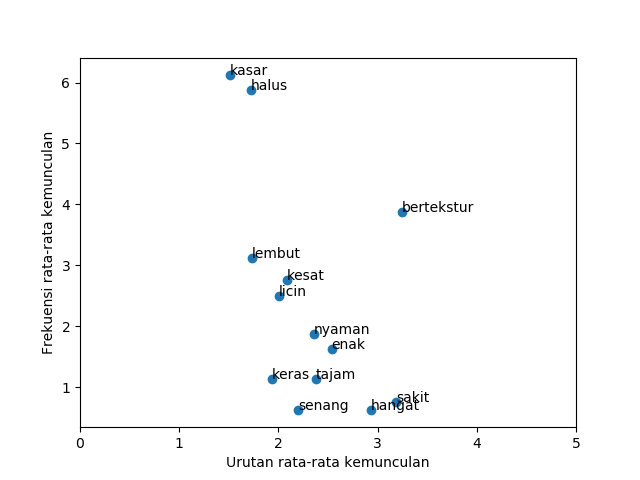
\includegraphics[scale=0.5]{gambar/grafik1}
		\caption{Grafik hubungan antara urutan rata-rata kemunculan dengan frekuensi rata-rata kemunculan terminologi afeksi}
		\label{grap11}
	\end{figure}
	\indent Korelasi antara frekuensi kemunculan rata-rata dan urutan kemunculan rata-rata dari suatu terminologi afeksi diuji menggunakan uji korelasi \emph{Pearson}. Dari uji korelasi \emph{Pearson} dengan $\alpha$(0.05) didapatkan nilai $P=0.077$. Berdasarkan hasil tersebut dapat diketahui bahwa tidak korelasi antara kemunculan rata-rata dengan frekuensi kemunculan rata-rata dari suatu terminologi afeksi.
	
	\subsection{Pemetaan Spasial Afeksi Pada Sentuhan}
	\indent Data dari hasil survey diproyeksikan pada bidang dua dimensi untuk diketahui klasifikasi material berdasarkan afeksi yang ditimbulkannya ketika disentuh. Proyeksi atau pemetaan yang dimaksud disini adalah \emph{plotting} material pada bidang dua dimensi berdasarkan data hasil survey yang telah diubah menjadi sebuah matriks persamaan untuk diketahui persamaan dari setiap material. 
	
		\begin{figure}[H]
		\centering
		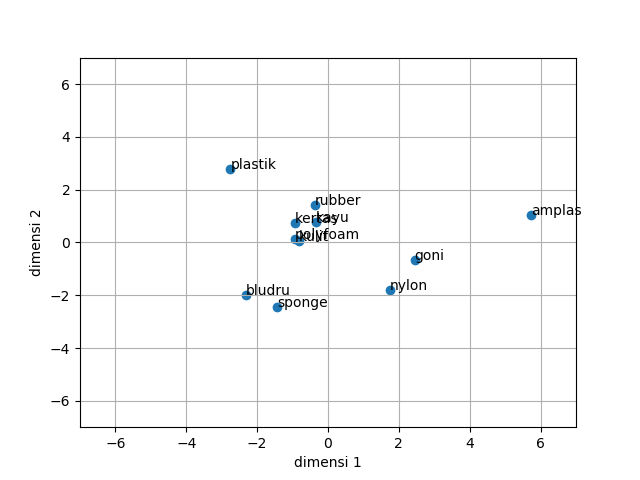
\includegraphics[scale=0.5]{gambar/plotmaterial.png}
		\caption{Plotting material berdasarkan afeksinya pada bidang 2 dimensi.}
		\label{plot_1}
	\end{figure}   
	\indent Berdasarkan Gambar 3.3 di atas secara visual dapat diketahui bahwa material dengan karakteristik riil yang sama berkelompok pada area yang sama. Ini terlihat dari material seperti amplas, nylon dan goni berada di sisi condong ke sebelah kanan. Sedangkan material seperti bludru, sponge serta plastik cenderung berada disisi sebelah kiri. Seperti yang kita ketahui bahwa kedua kelompok material ini memiliki sifat fisik yang cukup berlawanan. Sehingga dapat dikatakan bahwa pemetaan spasial dari material sudah dapat cukup merepresentasikan dengan kondisi yang sebenarnya termasuk juga untuk merepresentasikan aspek afeksi yang dimiliki oleh material tersebut.\\
	\indent Untuk mengetahui dimensi afeksi yang timbul dan dapat diproyeksikan pada bidang dua dimensi dibautlah vektor dimensi afeksi. Vektor ini didapatkan dari nilai koefisien $\beta$ hasil analisis \emph{multiple linear regression}. Vektor dimensi afeksi dapat dilihat dari Gambar 3.4 berikut.\\
	\begin{figure}[H]
		\centering
		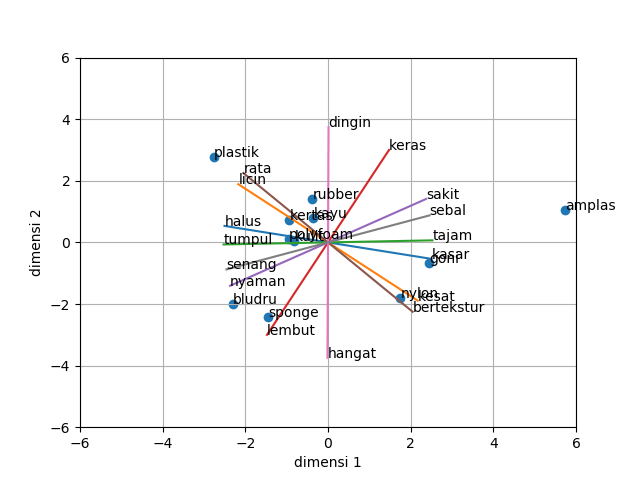
\includegraphics[scale=0.5]{gambar/mds1.png}
		\caption{Peta spasial dengan vektor dimensi afeksi.}
		\label{mds-1}
	\end{figure} 
	\indent Kesesuaian suatu dimensi afeksi untuk diproyeksikan pada suatu bidang ditunjukkan dari nilai koefisien determinasinya $R^2$. Koefisien determinasi $R^2$ didapatkan dari hasil analisis \emph{multiple linear regression}. Analisis \emph{multiple linear regression} menggunakan prediktor data dimensi satu dan dimensi dua sedangkan data targetnya adalah hasil survey dari dimensi afeksi yang dimaksud. Semakin tinggi nilai koefisien determinasinya maka semakin sesuai dimensi tersebut dalam peta spasial yang telah dibuat\cite{Holliins1993}. Seperti yang dapat dilihat dapat pada tabel berikut diketahui bahwa dimensi afeksi yang memiliki kesesuaian tertinggi adalah nyaman-sakit ($R^2$= 0.9675). Sedangkan dimensi afeksi dengan tingkat kesesuaian terendah adalah dingin-hangat ($R^2$= 0.8996).\\
	
		\begin{table}[H]
		\centering
		\caption{Nilai $R^2$ setiap dimensi afeksi.}
		\label{r21}
		\begin{tabular}{|c|c|c|}
			\hline
			No. & Afeksi & $R^2$\\
			\hline
			1 & Halus-Kasar & 0.9558\\
			\hline
			2 & Kesat-Licin & 0.9324\\
			\hline
			3 & Tajam-Tumpul & 0.9518\\
			\hline
			4 & Keras-Lembut & 0.9135\\
			\hline
			5 & Bertekstur-Rata&0.9621\\
			\hline
			6 & Nyaman-Sakit & 0.9675\\
			\hline
			7 & Dingin-Hangat & 0.8996\\
			\hline
			8 & Senang-Sebal& 0.9558\\
			\hline
		\end{tabular}
	\end{table}
	
	\indent Berdasarkan vektor dimensi yang berhasil diproyeksikan dapat diketahui hubungan antar dimensi afeksi sentuhan. Suatu dimensi dinyatakan memiliki hubungan apabila vektor dimensi afeksi memiliki hubungan kesejajaran \cite{Holliins1993}. Sedangkan apabila vektor dimensi saling tegak lurus maka dimensi afeksi diketahui saling berlawanan. Hubungan antar dimensi afeksi sentuhan yang dimaksud adalah dimensi afeksi timbul pada waktu hampir bersamaan ketika suatu permukaan material disentuh. Seperti yang dapat dilihat pada Gmabar 3.4 di atas mengenai vektor dimensi afeksi, diketahui bahwa vektor dimensi halus-kasar sejajar dengan tumpul-tajam. Selain itu dimensi afeksi nyaman-sakit sejajar dengan dimensi senang-sebal dan licin-kesat sejajar dengan rata-bertekstur. Dapat dilihat bahwa dimensi afeksi yang timbul ketika disentuh pada dasarnya memiliki kemiripan.

	\subsection{Pembuatan Model \emph{Machine Learning} Karakteristik Afeksi}
	\indent Pada eksperimen ini dilakukan dua langkah utama yaitu proyeksi data hasil ekstraksi fitur berbasis \emph{Fourier transform} pada bidang dua dimensi dan pembuatan model \emph{machine learning} beserta evaluasi performanya.\\ 
	\indent Dari eksperimen ini diketahui bahwa data hasil ekstraksi fitur berbasis \emph{Fourier transform} yang diproyeksikan pada bidang dua dimensi tidak sesuai dengan karakteristik riil dari material yang diekstraksi fiturnya. Ini diketahui dari hasil \emph{T-test} yang didapatkan nilai  $P<0.05$ ($P=0.000521$). Sehingga data hasil ekstraksi fitur berbasis \emph{Fourier transform} yang diproyeksikan pada peta spasial tidak dapat secara langsung karakteristik afeksi dari suatu material ketika disentuh. \\
	
	\begin{figure}[H]
		\centering
		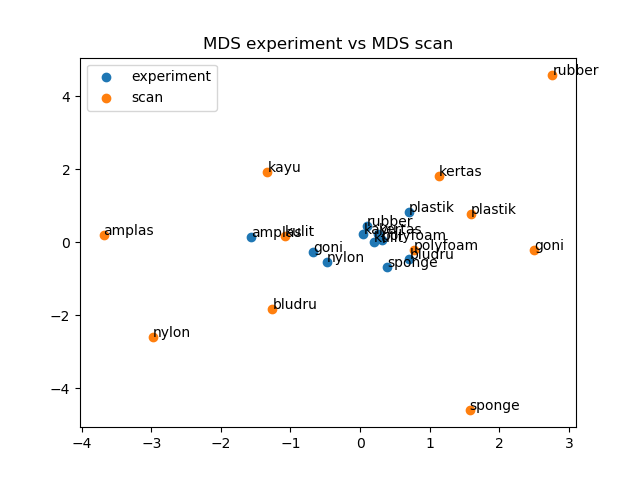
\includegraphics[scale=0.5]{gambar/scanexp}
		\caption{Grafik perbandingan hasil MDS eksperimen dan hasil scan}
		\label{scanvsexp1}
	\end{figure}

	\indent Model \emph{machine learning} yang digunakan pada eksperimen ini adalah \emph{Multi-Output Logistic Regression}. Performa dari model dievaluasi menggunakan beberapa parameter seperti nilai akurasi, kurva ROC dan validasi menggunakan data spesimen uji yang sebelumnya belum pernah dikenali oleh model yang dibuat. Berdasarkan evaluasi performa menggunakan nilai akurasi didapatkan hasil berupa tabel berikut. Dari tabel tersebut diketahui bahwa performa model berdasarkan nilai akurasi sangat baik untuk melakukan klasifikasi dimensi afeksi nyaman-sakit (0.9318). Sedangkan performa model buruk untuk melakukan klasifikasi dimensi afeksi keras-lembut (0.5909) dan dingin-hangat (0.6818).\\
	
	\begin{table}[H]
		\centering
		\caption{Akurasi model \emph{machine learning}.}
		\label{acc1}
		\begin{tabular}{|c|c|c|}
			\hline
			No & Afeksi & Akurasi \\
			\hline
			1 & Halus-Kasar & 0.8864\\
			\hline
			2& Kesat-Licin & 0.8181 \\
			\hline
			3&Tajam-Tumpul&  0.75 \\
			\hline
			4& Keras-Lembut&0.5909\\
			\hline
			5&Nyaman-Sakit&0.9318\\
			\hline
			6&Bertekstur-Rata&0.75\\
			\hline
			7&Dingin-Hangat&0.6818\\
			\hline
			8&Senang-Sebal&0.7273\\
			\hline
		\end{tabular}
	\end{table}
	
		\indent Model selanjutnya dievaluasi menggunakan kurva ROC untuk memastikan apakah benar nilai akurasi yang didapatkan dari model. Dapat dilihat dari kurva ROC yang didapat pada gambar dibawah ini diketahui bahwa kedua dimensi yang memiliki performa yang rendah pada evaluasi nilai akurasi juga terdeteksi pada kurva ROC. Sedikit perbedaan dari kurva ROC terlihat pada nilai ROC yang rendah pada dimensi afeksi kesat-licin (0.67). Ini sangat berkebalikan dengan evaluasi menggunakan nilai akurasi yang menunjukkan nilai akurasi dari dimensi kesat-licin (0.8181).\\
		
		\begin{figure}[H]
			\centering
			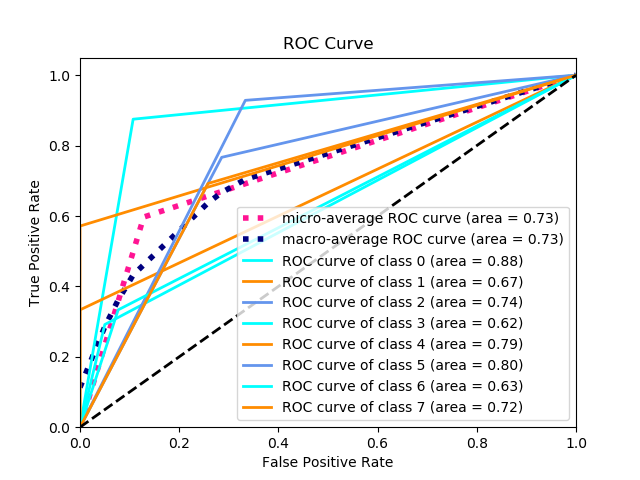
\includegraphics[scale=0.5]{gambar/roc}
			\caption{kurva ROC}
			\label{roc1}
		\end{figure}
	
	\indent Untuk evaluasi performa model menggunakan metode validasi data yang sebelumnya belum pernah diketahui bahwa model lemah dalam melakukan klasifikasi dan prediksi dimensi afeksi dingin-hangat, keras-lembut dan kesat-licin. Ini dikarenakan data yang didapatkan dari hasil survey menunjukkan karakteristik bahwa subjek mengalami kesulitan untuk melakukan klasifikasi pada dimensi afeksi yang disebutkan khususnya hangat-dingin. Sehingga ini mempengaruhi dari model mengingat bahwa data hasil survey digunakan sebagai data latih dari model yang dibuat. Selain itu dimensi afeksi dingin-hangat dan keras-lembut lebih sesuai untuk diproyeksikan pada bidang dua dimensi \cite{Picard2003}. Berikut adalah tabel hasil dari evaluasi model yang divalidasi dengan hasil survey.\\
	
		\begin{table}[H]
		\centering
		\caption{Hasil validasi model.}
		\label{val-mod1}
		\begin{tabular}{|c|c|c|c|}
			\hline
			No.& Afeksi &Bulu Sintetis & Kain \emph{suede}\\
			\hline
			1 & Halus-Kasar& 100\% & 80\% \\
			\hline
			2 & Kesat-Licin & 60\% & 80\% \\
			\hline
			3 & Tajam-Tumpul & 100\% & 100\% \\
			\hline
			4 & Keras-Lembut & 100\% & 40\% \\
			\hline
			5 & Nyaman-Sakit & 100\% & 100\% \\
			\hline
			6 & Bertekstur-Rata & 100\% & 40\% \\
			\hline
			7 & Dingin-Hangat& 100\% & 0\% \\
			\hline
			8 & Senang-Sebal& 100\% & 100\% \\
			\hline
			
		\end{tabular}
	\end{table}

	\section{Pembahasan}
	\indent Pada penelitian ini terdapat tiga eksperimen yang setiap eksperimen saling berkaitan. Eksperimen pertama adalah eksperimen pengumpulan terminologi afeksi sentuhan. Kajian utama yang dikaji pada eksperimen ini adalah terminologi yang digunakan seseorang dalam menyampaikan kesan afeksi yang timbul ketika menyentuh suatu permukaan material. Berdasarkan eksperimen ini diketahui bahwa secara umum terdapat dua jenis terminologi afeksi yaitu terminologi afeksi terkait dengan karakteristik fisik dan terminologi yang terkait dengan aspek emotif. Terminologi afeksi terkait dengan karakteristik fisik seperti halus, kasar, kesat, licin, bertekstur, rata, tajam, tumpul, keras, lembut, dingin dan hangat. Sedangkan untuk terminologi terkait dengan karakteristik emotif yang muncul yaitu nyaman, sakit, senang dan sebal.\\
	\indent Selain itu pada eksperimen pengumpulan terminologi afeksi juga diketahui bahwa jenis kelamin tidak mempengaruhi perbedaan kemampuan semantik dalam menyampaikan kesan dari afeksi pada sentuhan. Berdasarkan ini dapat diketahui bahwa tidak ada variasi yang cukup beragam dalam penyampaian kesan afeksi sentuhan dengan suatu terminologi. Hal ini perlu diteliti lebih lanjut mengenai mekanisme terbentuknya suatu terminologi untuk menyampaikan suatu konsep.\\
	\indent Eksperimen ini juga mengumpulkan data berupa frekuensi kemunculan rata-rata dan urutan kemunculan rata-rata. Dari kedua data tersebut dicari korelasi apakah ada pengaruh antara urutan kemunculan rata-rata suatu terminologi dengan frekuensi kemunculan rata-rata. Dari eksperimen ini didapatkan hasil bahwa urutan kemunculan rata-rata tidak berkorelasi dengan frekuensi kemunculan rata-rata dari suatu terminologi afeksi menggunakan uji korelasi \emph{Pearson}.\\
	\indent Eksperimen kedua berusaha meneliti tentang pemetaan spasial afeksi pada sentuhan. Afeksi yang berusaha dipetakan pada eksperimen ini adalah terminologi afeksi yang didapatkan dari ekperimen pertama. Material spesimen dipetakan pada bidang dua dimensi berdasarkan afeksi yang ditimbulkannya ketika disentuh. Sehingga dapat material spesimen uji dapat berkelompok dengan material yang memiliki afeksi yang sama.\\
	\indent Material spesimen uji yang sudah dipetakan berdasarkan afeksinya dapat diketahui dimensi afeksi yang muncul. Di antara dimensi afeksi yang muncul tersebut ditemukan hubungan antar dimensi. Hubungan ini diketahui dengan vektor dimensi afeksi yang saling sejajar. Vektor dimensi afeksi seperti halus-kasar dengan tumpul-tajam, nyaman-sakit dengan senang-sebal dan licin-kesat dengan rata-bertekstur memiliki hubungan kesejajaran. Hal ini berindikasi bahwa dimensi afeksi yang saling sejajar saling berhubungan atau dapat dikatakan bahwa kedua dimensi tersebut memiliki karakteristik yang serupa.\\
	\indent Eksperimen ketiga dilakukan untuk membuat model \emph{machine learning} untuk mengetahui karakteristik afeksi pada sentuhan. Model yang digunakan pada eksperimen ini adalah \emph{Multi-Output Logistic Regression}. Dari model ini diketahui performa model kurang baik untuk melakukan klasifikasi dan prediksi afeksi dingin-hangat dan keras-lembut.\\
	\indent Fitur berbasis \emph{Fourier transform} dipetakan kedalam bidang dua dimensi dan dibandingkan dengan hasil pemetaan afeksi hasil eksperimen kedua. Diketahui dari eksperimen ini bahwa fitur berbasis \emph{Fourier transform} yang diproyeksikan pada bidang dua dimensi tidak dapat digunakan untuk menentukan afeksi yang timbul dari suatu permukaan ketika disentuh.\\

	\section{Kesimpulan}
	\indent Berdasarkan penelitian ini dapat ditarik kesimpulan sebagai berikut:
	\begin{enumerate}
		\item Terdapat macam-macam aspek afeksi dari suatu permukaan seperti halus-kasar, kesat-licin, keras-lembut, bertekstur-rata, tajam-tumpul, nyaman-sakit, dingin-hangat dan senang-sebal.
		
		\item Terdapat hubungan antar dimensi afeksi yang ada pada suatu permukaan. Diketahui bahwa dimensi afeksi halus-kasar sejajar dengan tumpul-tajam. Ini juga terjadi pada dimensi afeksi nyaman sakit sejajar dengan afeksi senang-sebal.
		
		\item Afeksi sentuhan dari suatu permukaan tidak dapat langsung diketahui dari fitur berbasis \emph{Fourier transform} yang dipetakan pada bidang dua dimensi.
		
		\item Model yang dapat digunakan untuk mengetahui hubungan antara karakteristik afketif berbasis \emph{Fourier transform} adalah \emph{Multi-Output Logistic Regression}. Performa model yang dibuat memiliki tingkat akurasi yang cukup tinggi untuk klasifikasi afeksi halus-kasar (88.64\%), kesat-licin (81.81\%), tajam-tumpul (75\%), nyaman-sakit (93.18\%), bertekstur-rata (75\%) dan senang-sebal (72.73\%). Sedangkan model yang dibuat memiliki performa akurasi yang rendah untuk mengklasifikasi dimensi afeksi keras-lembut (59.09\%) dan dingin-hangat (68.18\%). Karakteristik serupa ditemui pada evaluasi performa menggunaka kurva ROC namun ditambah bahwa model lemah dalam melakukan klasifikasi dimensi kesat-licin dengan nilai ROC (0.67).
	\end{enumerate}
	
	\section{Saran}
	\indent Untuk penelitian selanjutnya disarankan untuk: 
	\begin{enumerate}
		\item Untuk penelitian selanjutnya disarankan untuk melakukan penelitian mengenai mekanisme munculnya terminologi afeksi. Ini diperlukan untuk mengetahui bagaimana manusia menyampaikan suatu konsep yang dipahaminya dan bagaimana manusia memilih suatu terminologi untuk mewakili konsep yang dipahaminya.    
		\item Disarankan untuk penelitian selanjutnya citra digital sebelum diekstraksi fiturnya dilakukan proses SVD terlebih dahulu. 
		\item Pada penelitian selanjutnya diharapkan untuk pemetaan spasial untuk menggunakan proyeksi pada bidang tiga dimensi atau lebih. 
		\item Pada penelitian selanjutnya diharapkan untuk dapat menambah jumlah data guna meningkatkan performa dari model yang dibuat.
	\end{enumerate}
	\bibliography{daftarpustaka.bib}
	
\end{multicols}

\end{document}